%! Author = naza
%! Date = 3/10/25

% Preamble
\documentclass[a4paper,oneside,12pt]{amsart}

% Packages
\usepackage{amsmath}
\usepackage{latexsym}
\usepackage{multicol}
\usepackage{enumerate}
\usepackage{enumitem}
\usepackage[heightrounded]{geometry}
\geometry{top=2cm,bottom=2cm,left=2cm,right=2cm}
\usepackage{graphicx}
\newcommand{\xopt}{x^{*}}
\newcommand{\yopt}{y^{*}}
\newcommand{\zopt}{z^{*}}
\theoremstyle{definition}
\newtheorem{quest}{Ejercicio}
\thispagestyle{empty}
\usepackage{tikz}
\usetikzlibrary{automata,positioning}

% Document
\begin{document}

    \begin{quest}
        \item \begin{enumerate}[label=\alph*)]
                  \item  Problema dual:
                  \[
                        \begin{array}{rrcrcrcr}
                            \min & -4y_1 & - & 2y_2 & - & y_3 & & \\
                            \text{s.a:} & y_1 &  &  & + & y_3 & \leq & 3\\
                            & 2y_1 & - & y_2 & + & y_3 & = & 2\\
                            & y_1 & - & y_2 &  & & \leq & 2\\
                            & \multicolumn{5}{r}{y} & \geq & 0 \\
                        \end{array}
                        \]
                  \item \textbf{Fase I:} estandarizamos el problema para Fase I:
                  \[
                        \begin{array}{rrcrcrcrcr}
                            \max & -a_1 & & & & & & \\
                            \text{s.a:} & y_1 &  &  & + & y_3 & + & w_1 & = & 3\\
                            & 2y_1 & - & y_2 & + & y_3 & + & a_1 & = & 2\\
                            & y_1 & - & y_2 &  & & + & w_2 & = & 2\\
                            & \multicolumn{7}{r}{y,a_1,w} & \geq & 0 \\
                        \end{array}
                        \]
                  Resolvemos:
                          \[
                            \begin{array}{rcllll}
                            w_1 & =  &3 &-y_1 &  &-y_3\\
                            w_2 & =  &2 &-y_1 &+y_2 & \\
                            a_1 & =  &2 &-2y_1 &+y_2 &-y_3\\\hline
                            z &= &-2 &+2y_1 &-y_2 &+y_3\\
                            \end{array}
                            \]
                            \vspace{1cm}
                            \[
                            \begin{array}{rcllll}
                            w_1 & =  &2 &-1/2y_2 &-1/2y_3 &+1/2a_1\\
                            w_2 & =  &1 &+1/2y_2 &+1/2y_3 &+1/2a_1\\
                            y_1 & =  &1 &+1/2y_2 &-1/2y_3 &-1/2a_1\\\hline
                            z &= &  &  &  &-a_1\\
                            \end{array}
                            \]

                  \textbf{Fase II:} escribimos el primer diccionario de la Fase II y resolvemos
                    \[
                    \begin{array}{rclll}
                    y_1 & =  &1 &+1/2y_2 &-1/2y_3\\
                    w_1 & =  &2 &-1/2y_2 &-1/2y_3\\
                    w_2 & =  &1 &+1/2y_2 &+1/2y_3\\\hline
                    z &= &4 &+4y_2 &-y_3\\
                    \end{array}
                    \]
                    \vspace{1cm}
                    \[
                    \begin{array}{rclll}
                    y_1 & =  &3 &-y_3 &-w_1\\
                    w_2 & =  &3 &  &-w_1\\
                    y_2 & =  &4 &-y_3 &-2w_1\\\hline
                    z &= &20 &-5y_3 &-8w_1\\
                    \end{array}
                    \]
                    \vspace{1cm}
                    \textbf{Solución del dual:} $y^\ast = (3, 4, 0)$
                  \item Aplicamos Teorema de Holgura Complementaria:
                    \[
                  \begin{array}{rl}
                      y_1^\ast - y_2^\ast < 2 & \Rightarrow x_3^\ast = 0 \\
                      y_1^\ast \neq 0 & \Rightarrow \xopt_1+2\xopt_2+\xopt_3 = -4 \\
                      \yopt_2 \neq 0 & \Rightarrow -\xopt_2 - \xopt_3 = -2 \\
                  \end{array}
                  \]
                  Tenemos entonces que:
                  \[
                      \begin{cases}
                          \xopt_1+2\xopt_2= -4 \\
                          -\xopt_2 = -2
                      \end{cases}
                      \Rightarrow \xopt = (-8,2, 0)
                  \]
        \end{enumerate}
    \end{quest}

    \begin{quest}\hphantom{1em}

        \begin{enumerate}[label=\alph*)]
            \item \textbf{Verdadero}: como $d>e>0$, $x_1$ entra a la base y, como $b>0$ y $\frac{1}{b}<\frac{a}{2}$,
            podemos deducir que $a>0$. Luego, la restricción más ajustada al crecimiento de $x_1$ está dada por
            $x_5\geq 0$, por lo que esa variable sale de la base.
            \item Ambiguo, consideremos dos respuestas correctas:

            \textbf{Falso}: si $d\leq0$ y $e\leq 0$ no hay próxima iteración.

            \textbf{Verdadero}: si $x_1$ entra a la base, la restricción $x_4\geq 0$ hace que $x_1$ deba valer $0$.
            Si $x_3$ entra a la base, la restricción $x_4\geq 0$ obliga que $x_3$ no pueda aumentar su valor.
            \item \textbf{Verdadero:} como $d=0$ y $e\leq 0$, el diccionario corresponde a una solución básica óptima.
            Además, $x_1$ puede tomar cualquier valor en $[0, m]$ donde:
            \[m = \begin{cases}
               \min\{\frac{2}{a}, \frac{1}{b}\} & \text{si $b>0$} \\
                      \frac{2}{a}               & \text{si $b \leq 0$}
            \end{cases}\]
            y el valor de la f.o. sigue siendo el mismo.
            \item \textbf{Falso:} Como $e>d>0$, $x_3$ entra a la base. Aunque $c>0$, $x_3$ puede crecer hasta
            $\min\{2a, \frac{2}{3}\}$, por lo tanto, no son condiciones necesarias para que el problema sea no acotado.
        \end{enumerate}
    \end{quest}

    \begin{quest}\hphantom{1em}

        \textbf{Poliedro de la relajación lineal:}
        \begin{figure}[htbp!]
            \centering
            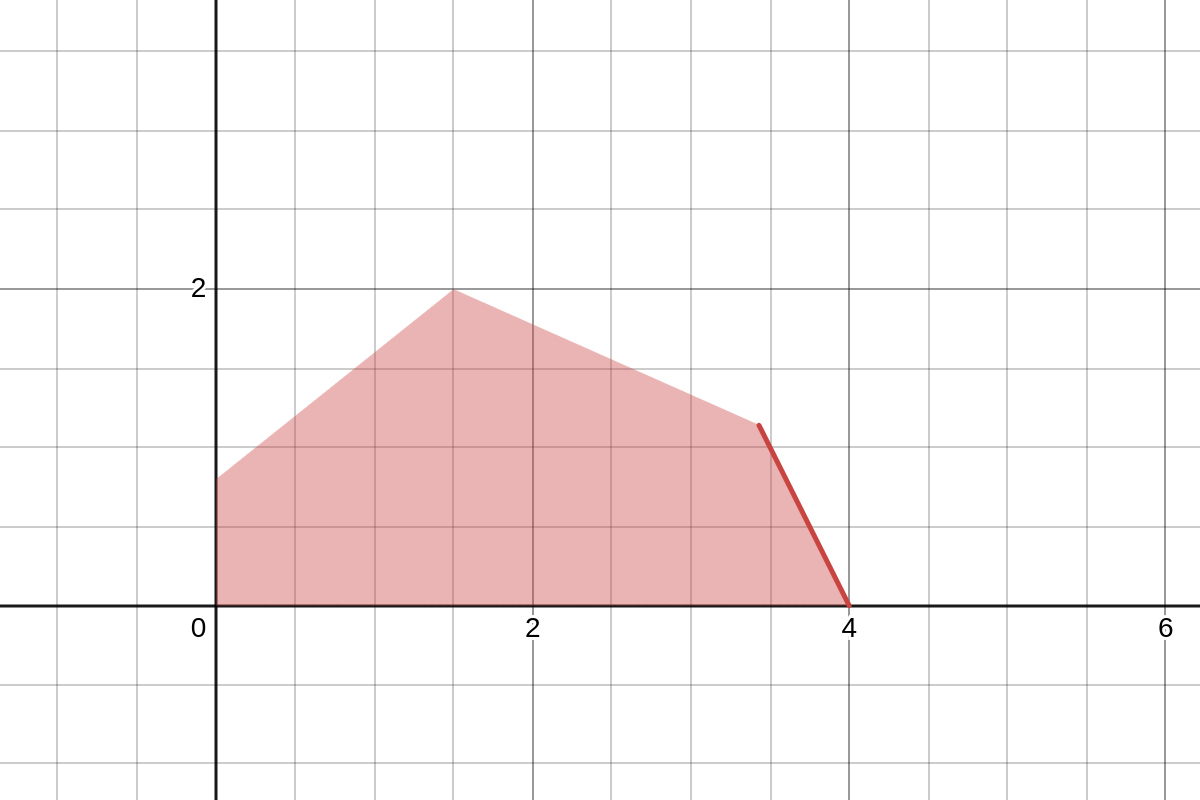
\includegraphics[width=0.9\textwidth]{BB_region}
        \end{figure}

       \textbf{Árbol de B\&B:}

        \begin{figure}
            \centering
            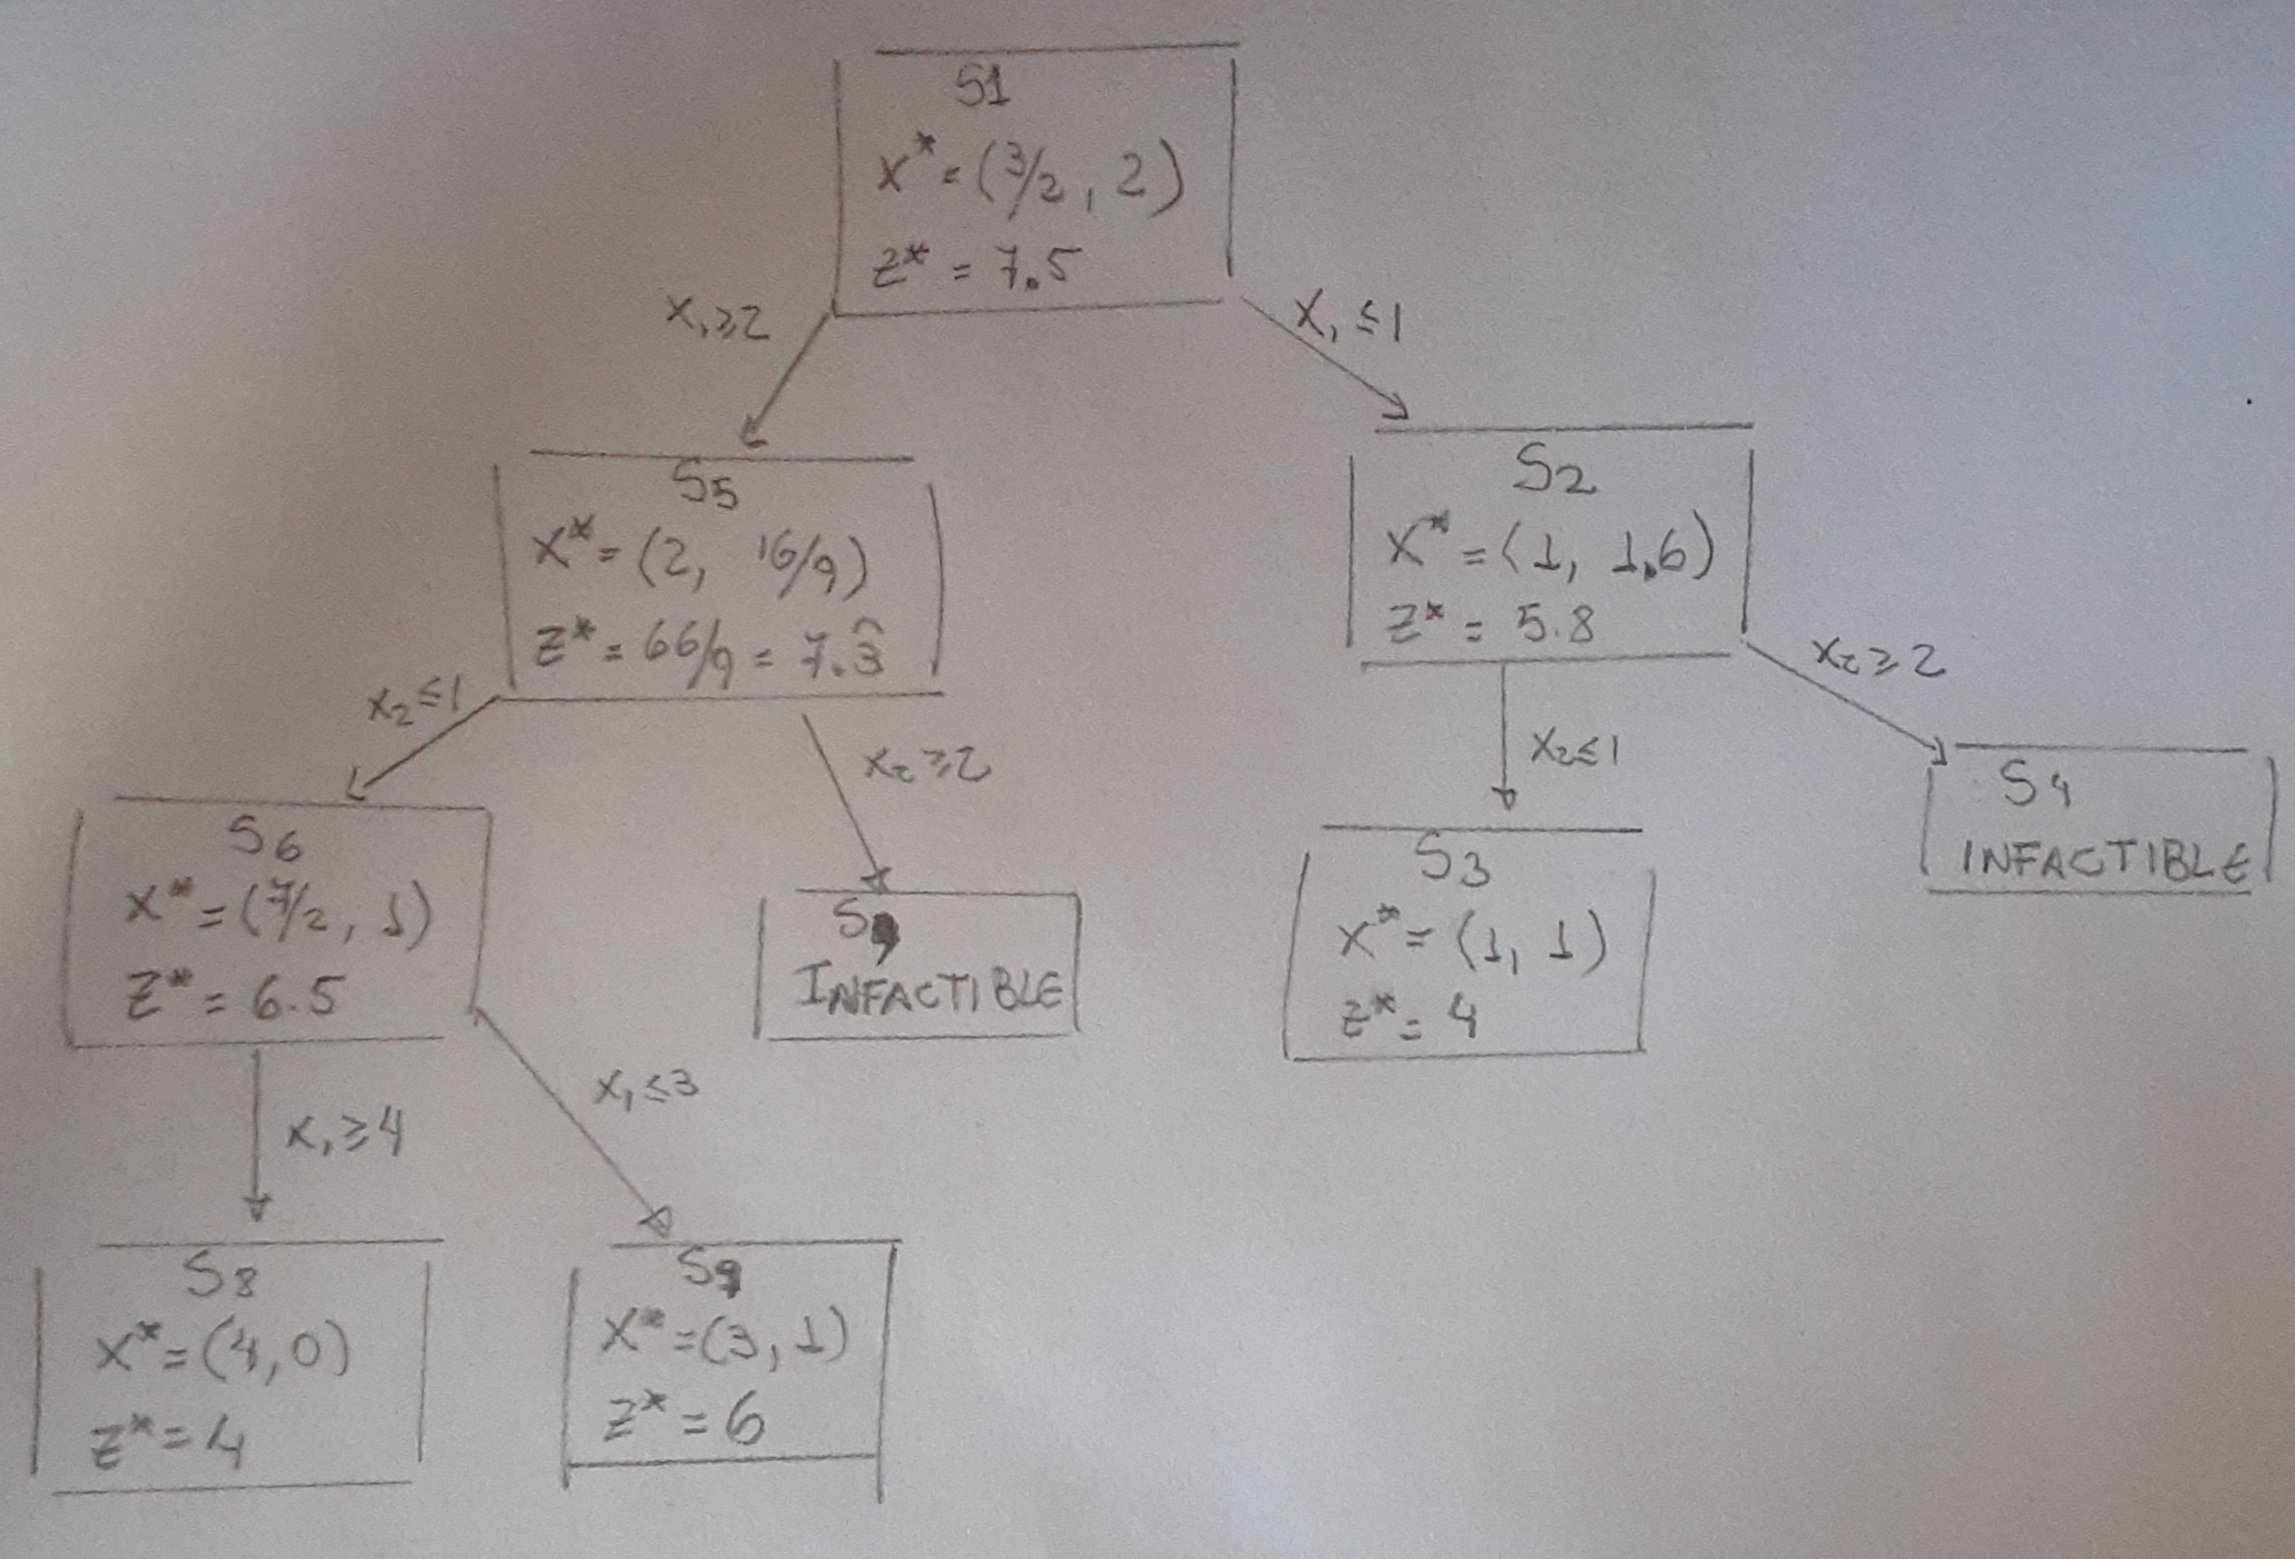
\includegraphics[width=\textwidth]{Arbol_BB_manual}
        \end{figure}
    \end{quest}
\end{document}